\onehalfspacing

Previous models of the UIFESS focused on the bearing aspects of the machine. The project had need of a model that could predict torque production and dynamically respond to both changes in position and current distribution. This model also needed to be capable of determining the effects of non-ideal materials being used in the rotor. It is also advantageous for the model to predict the losses due to saturation and the effects of mechanical deformation of the rotor.


What were we trying to accomplish?
	A model that is flexible enough to use in the development process to determine the best path forward for the machine. 
	
	In the model we desired the ability to predict the bearing forces and torque due to stator and rotor configurations.
	
	We wish to be able to predict the losses due to saturation and deflection.
	
	

\section{Torque Production}
The torque production in the model is determined by taking the derivative of the air gap energy with respect to the displacement angle.

\section{MATLAB\textsuperscript{\textregistered} Development}
Pain in my ass

\section{Effects of Non Ideal Materials}
The future of the UIFESS is dependent on the ability of the machine to reach high rotational velocities. The mechanical limitations of this design criterion and some solutions are discussed in \cite{Pettingill}.  To overcome the mechanical limitations carbon fiber and iron composts were evaluated to determine both mechanical and electromagnetic properties.

The electrical limitations are evident in the permeability of the materials. The permeability of the composts was found to be much less than that of the iron due to the air gap effect created by the matrix and carbon fibers. This reduction in permeability will effect both the machines ability to produce correctional forces and torque.

The effect on bearing forces can be expressed through the force equation derived from amperes law or magnetic equivalent circuits. The magnetic circuit in Figure \ref{fig:SimpleMagneticCircuit} was created with the assumption that the horse shoe and floater are composed of iron. The assumptions that the two components are iron and that the permeability of iron is always much greater than 1 leads to the derivation presented in \cite{Wimer}. This derivation results in the simplification of equation \ref{Eq:BwFe} into equation \ref{Eq:BwoFe}. In the ensuing discussion, $ni$ or magnetomotive force (MMF) will be represented as $NI$.

\begin{figure}[!t]
	\centering
	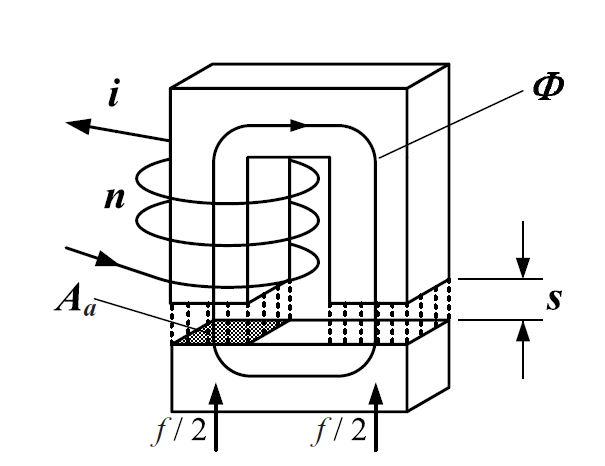
\includegraphics[width=4in]{./Pictures/SimpleMagneticCircuit.jpg}
	\caption{A simple magnetic circuit, from \cite{MagBear}}
	\label{fig:SimpleMagneticCircuit}
\end{figure}

\begin{equation}\label{Eq:BwFe}
B={\mu }_{0}\frac{NI}{\Big(\frac{l_{fe}}{{\mu }_{r}}+2s\Big)}
\end{equation}

\begin{equation}\label{Eq:BwoFe}
B={\mu }_{0}\frac{NI}{2s}
\end{equation}

If the horse shoe and the floater are not made of the same material then the equations needs to be modified starting with equation \ref{Eq:AmpLaw} where the floater is assumed to be made of a composite material. 

\begin{equation}\label{Eq:AmpLaw}
\underset{l}{\oint }\stackrel{-}{H}\cdot d\stackrel{-}{s}={l}_{fe}{H}_{fe}+2s{H}_{a}+{l}_{c}{H}_{c}=NI
\end{equation}

Also assuming that the flux $\Phi$ follows a path within the magnetic loop and that the cross sections of each material are equal, the flux density $B$ can be computed from the following equations \cite{MagBear}. Where

\begin{equation}\label{Eq:BwFe}
\Phi={A}_{fe}{B}_{fe}={A}_{a}{B}_{a}={A}_{c}{B}_{c}
\end{equation}
 and
\begin{equation}\label{Eq:BwoFe}
{A}_{fe}={A}_{a}={A}_{c}
\end{equation}
therefore
\begin{equation}\label{Eq:BwFe}
{B}_{fe}={B}_{a}={B}_{c}=B
\end{equation}

% ADD DISCUSSION ABOUT THE EFFECTS OF leakage flux


Since the flux density is identical in each of the materials, the field intensities ${H}_{fe}$, ${H}_{a}$, and ${H}_{c}$ from equation \ref{Eq:AmpLaw} can be replaced as shown in equation \ref{Eq:MMFwB}:

\begin{equation}\label{Eq:MMFwB}
{l}_{fe}\frac{B}{{\mu}_{0}{\mu}_{fe}}+2s\frac{B}{{\mu}_{0}}+{l}_{c}\frac{B}{{\mu}_{0}{\mu}_{c}}=NI
\end{equation}

Solving equation \ref{Eq:MMFwB} for $B$ yields

\begin{equation}\label{Eq:B}
B={\mu}_{0}\frac{NI}{\Big(\frac{{l}_{fe}}{{\mu}_{fe}}+2s+\frac{{l}_{c}}{{\mu}_{c}}\Big)}
\end{equation}

% ADD DISCUSSION ABOUT THE EFFECTS OF SATURATION ON B

The attraction force of an electromagnet is generated at the boundaries between differing permeability and can be calculated based on the field energy \cite{MagBear}.  The energy stored in the volume of the air gap can be expressed as

\begin{equation}\label{Eq:Wa}
{W}_{a}=\frac{1}{2}{B}_{a}{H}_{a}{V}_{a}=\frac{{{B}_{a}}^{2}{V}_{a}}{2{\mu}_{0}}
\end{equation}
where
\begin{equation}\label{Eq:Va}
{V}_{a}=2s{A}_{a}
\end{equation}

The force acting on the floater is generated by a change in the air gap field energy. This can be expressed as a function of the floater displacement. If the displacement is small the magnetic flux remains constant and an increase in displacement will result in an increase in energy \cite{MagBear}. Using the principle of virtual displacement, where the system is frozen in time and one degree of freedom is displaced by a small amount \cite{AnaMech}, the force can be expressed as the partial derivative of the field energy with respect to the air gap \cite{MagBear}.

\begin{equation}\label{Eq:F}
f=-\frac{\partial {W}_{a}}{\partial s}=\frac{{{B}_{a}}^{2}{A}_{a}}{{\mu}_{0}}
\end{equation}

By combining equation \ref{Eq:F} and equation \ref{Eq:B}, the force on the floater can be expressed as a function of the coil current and air gap.

\begin{equation}\label{Eq:Fwis}
f={\mu}_{0}{A}_{a}{\left[\frac{NI}{\Big(\frac{{l}_{fe}}{{\mu}_{fe}}+2s+\frac{{l}_{c}}{{\mu}_{c}}\Big)}\right]}^{2}
\end{equation}

This function is useful for the horse shoe configuration shown in Figure \ref{fig:SimpleMagneticCircuit} but needs to be modified for use with a cylindrical configuration as would be used with a machine. For a curved surface, like the one shown in Figure \ref{fig:CurvedMagneticCircuit},  $A_a$ is assumed to be the projected area of the pole face \cite{MagBear}. Also the angel $\alpha$ must be considered in determining the force and is dependent on the number of poles the machine has. Equation \ref{Eq:Fwis} can be modified with these considerations to produce:

\begin{figure}[!t]
	\centering
	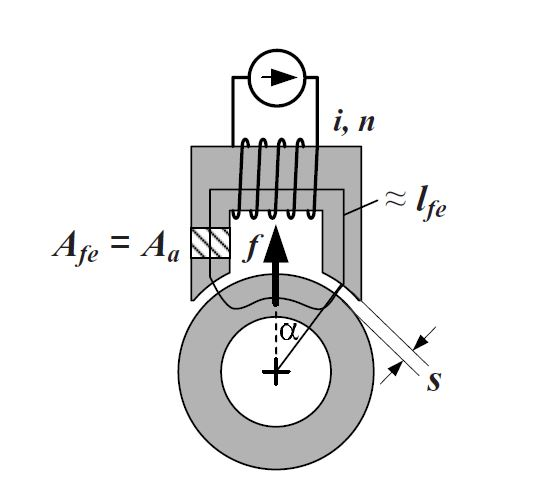
\includegraphics[width=4in]{./Pictures/CircularMagneticCircuit.jpg}
	\caption{A cylindrical magnetic circuit, from \cite{MagBear}}
	\label{fig:CurvedMagneticCircuit}
\end{figure}

\begin{equation}\label{Eq:FwisAlpha}
f={\mu}_{0}{A}_{a}{\left[\frac{NI}{\Big(\frac{{l}_{fe}}{{\mu}_{fe}}+2s+\frac{{l}_{c}}{{\mu}_{c}}\Big)}\right]}^{2}\cos(\alpha)
\end{equation}

% ADD discussion on linearization and control 

% ADD discussion on magnetic equivalent circuits 

For this model to be used in the future of the UIFESS it needs to be both verified and validated. Verification of the model was performed by using another magnetic circuit modeling technique to determine whether the results are appropriate under the assumptions made. The modeling technique used is the gyrator-capacitor model developed by Buntenbach in the late 1960's. This technique uses MMF ($\mathcal{F}$) as a effort variable and rate of change of flux ($\frac{d\Phi }{dt}\equiv\stackrel{.}{\Phi}$) as a flow variable. Under this variable scheme magnetic permeance ($\mathcal{P}$) is analogous to electrical capacitance, and can be calculated using equation \ref{Eq:Perm}, where $A$ is cross section area and $\ell$ is member length \cite{GyrCapApp}.

\begin{equation}\label{Eq:Perm}
\mathcal{P}={\mu}_{0}{\mu}_{r}\frac{A}{\ell}
\end{equation}

\begin{figure}[t]
	\centering
		\begin{picture}(150,240)
			\put(0,0){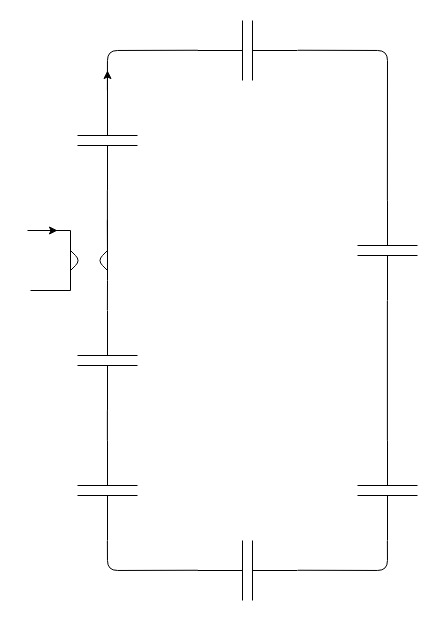
\includegraphics[width=2in]{./Pictures/Gyrator-CapApp.jpg}}
			\put(25,171){$\stackrel{.}{\Phi}$}
			\put(36,148){$\mathcal{P}_{fe1}$}
			\put(24,130){$N$}
			\put(12,130){$i$}
			\put(36,125){$+$}
			\put(36,115){$\mathcal{F}$}
			\put(36,107){$-$}
			\put(0,125){$+$}
			\put(0,115){$v$}
			\put(0,107){$-$}
			\put(36,75){$\mathcal{P}_{fe2}$}
			\put(36,32){$\mathcal{P}_{a}$}
			\put(85,8){$\mathcal{P}_{c}$}	
			\put(130,32){$\mathcal{P}_{a}$}		
			\put(130,112){$\mathcal{P}_{fe3}$}
			\put(85,180){$\mathcal{P}_{fe4}$}			
		\end{picture}
		\caption{A gyrator-capacitor model of a simple magnetic circuit}
		\label{fig:GyratorCapModel}
\end{figure}

The magnetic circuit shown in Figure \ref{fig:SimpleMagneticCircuit} can be represented as the gyrator-capacitor model shown in Figure \ref{fig:GyratorCapModel}. Where $\mathcal{P}_{fe}$, $\mathcal{P}_{a}$, and $\mathcal{P}_{c}$ are the permeance of iron, air, and a composite respectively. A distinct feature of this approach is that windings are treated as two port elements linking the electrical and magnetic circuits \cite{GyrCapApp}. The gyrator can be described using the following equations:

\begin{equation}\label{Eq:GyrV}
v=N\stackrel{.}{\Phi}
\end{equation}

\begin{equation}\label{Eq:GyrI}
i=\frac{\mathcal{F}}{N}
\end{equation}

Once the model is generated it can be analyzed as a capacitive circuit. In order to verify the force model represented in equation \ref{Eq:Fwis} the energy stored in the two $\mathcal{P}_{a}$ capacitors must be calculated, this represents the air gap energy. The energy stored in the air gap capacitor can be calculated using equation \ref{Eq:CapW}, where $\mathcal{F}_{a}$ is the MMF across the air gap.

\begin{equation}\label{Eq:CapW}
W_{a}=\frac{1}{2}\mathcal{P}_{a}{\mathcal{F}_{a}}^{2}
\end{equation}

Equation \ref{Eq:CapW} requires the calculation of the MMF across the air gap:

\begin{equation}\label{Eq:CapV}
\mathcal{F}_{a}=\frac{1}{\mathcal{P}_{a}}\left[{\int}_{{t}_{0}}^{\tau }\stackrel{.}{\Phi}dt+\mathcal{F}_{a0}\right]
\end{equation}

Then the force can be calculated by taking the partial derivative of the air gap energy with respect to the change in the air gap. Unfortunately this model does not simplify to a simple equation that represents the force as a function of the air gap and current. The model can be solved using a variety of softwares such as LTSpice\textsuperscript{\textregistered} or MATLAB\textsuperscript{\textregistered}. 

% ADD Discussion on the results of the two models

% ADD Discussion on the need for validation




% ADD Discusion on the benefits of each model.



